%%%%%%%%%%%%%%%%%%%%%%%%%%%%%%%%%%%%%%%%%%%%%%%%
% COPYRIGHT: (C) 2020 FAU FabLab
% CC-BY-SA 3.0
%%%%%%%%%%%%%%%%%%%%%%%%%%%%%%%%%%%%%%%%%%%%%%%%


\newcommand{\basedir}{fablab-document}
\documentclass{\basedir/fablab-document}

\renewcommand{\texteuro}{\euro}

\renewcommand{\todo}[1]{\textbf{\color{red}{TODO: #1}}}
\newcommand{\pfeil}{\ensuremath{\rightarrow}}

\date{2020}
\author{}
\fancyfoot[L]{kontakt@fablab.fau.de}
\title{Einweisung Nähmaschine Pfaff 260}


\begin{document}
\maketitle

\section{Grundlagen}

\subsection{Vor dem Nähen}
\begin{itemize}
	\item Nähmaschine auf einen stabilen Tisch stellen, sodass sie \textbf{nicht wackelt}
	\item Haube abnehmen, indem du die seitlichen Schnallen an der Basis der Nähmaschine löst und die Haube nach oben abziehst
	\item Einen \textbf{kleinen(!)} Tropfen Nähmaschinen- bzw. Feinmechaniknöl an der richtigen Stelle auf den Umlaufgreifer geben. Überschüssiges Öl sofort abwischen.
	\item \textbf{ACHTUNG: Die Nähmaschine ist sofort nähbereit, nachdem an den Strom angesteckt wurde. Der Schalter auf der rechten Seite schaltet lediglich das Nählicht ein und aus.}
	\item Netzkabel mit Fußanlasser anschließen, indem du es \textbf{zuerst(!)} mit der Nähzmaschine verbindest und \textbf{danach(!)} in eine Steckdose steckst 
\end{itemize}

\subsection{Nach dem Nähen}
\begin{itemize}
	\item Nähmaschine ausschalten indem du das Netzkabel \textbf{zuerst(!)} aus der Steckdose ziehst und \textbf{danach(!)} von der Maschine trennst
	\item Fußanlasser aufräumen
	\item Stoffstück unter Nähfuß legen und diesen dann abgesenken
	\item Transporthaube auf Maschine setzen und mit den seitlichen Schnallen an der Basis der Nähmaschine befestigen
	\item Nähmaschine aufräumen
	\item Sonstiges Zubehör, Garn, usw. wieder an seinen Platz verräumen
	\item Garn- und Stoffreste und Fusseln, die beim Nähen und Schneiden von Textilien auf dem Tisch entstehen wegfegen und in einen Mülleimer werfen. Danach alles, was auf den Boden gefallen ist aufsaugen.
\end{itemize}

\pagebreak

\subsection{Regeln und Hinweise}
\begin{itemize}
	\item Achte immer darauf, wo sich deine Finger befinden. Die Maschine näht viel schneller, als du im Notfall reagieren kannst. Nimm beim hantieren im Nähbereich immer den Fuß vom Anlasser. Achte beim Nähen darauf, immer genug Abstand zwischen der Nadel und deinen Händen zu halten.
	\item Für jede Näharbeit solltest du immer eine richtige und einwandfreie, nicht verbogene Nadel verwenden. Bei der Verwendung einer verbogenen Nadel, kann diese auf die Stichplatte treffen und dadurch der Mechanik der Maschine stark beschädigt werden.
	\item Den Stoff niemals schieben oder ziehen. Den Transport der Stoffes erledigt der sog. Transporteur für dich. Du musst musst lediglich den Stoff um die Nadel herum drehen, um die Richtung vorzugeben. Solltest du dennoch am Stoff ziehen oder ihn schieben, kann sich die Nadel mit den oben genannten Folgen verbiegen
	\item Nähe nie bei beschädigter Stichplatte, sonst kann sich die Nadel verbiegen/brechen (s.o.).
	\item Bevor du losnähst, achte immer darauf, dass der Nähfuß abgesenkt ist. Der Nähfuß lässt sich mit dem Nähfußheber an der Rückseite der Maschine heben und senken. Solltet ihr bei angehobenem Nähfuß losnähen, werder ihr Fadensalat produzieren, der u.U. nur sehr aufwändig wieder entfernt werden kann.
	\item Nichts mit Gewalt verschieben, einsetzen, bewegen, verstellen! Die Mechanik ist bei korrekter Handhabung und Behandlung leichtgängig.
	\item Verschiedene Materialien erfordern die Verwendung verschiedener Nadelstärken (üblicherweise zwischen 60 und 110) und Nadeltypen (z.B. Stretch-, Jeans-,  Universalnadel, etc.)
	\item Ohne Rücksprache mit einem Betreuer darf niemals die Unterfadenspannung verändert werden.
	\item Achte beim Nähen immer darauf, wie sich die Maschine verhält. Geräusche, Gerüche, Nadelbewegung oder Vibrationen, die dir bisher unbekannt waren, können auf Beschädigungen an der Maschine oder eine Fehlbedienung hinweisen. Bitte informiere immer eine:n Betreuer:in, wenn dir etwas komisch vorkommt.
	\item Das Nählicht der Maschine wird mit Netzspannung (230V) betrieben. Die Glühbirne darf daher niemals bei in die Steckdose eingesteckter Maschine gewechselt werden. Andern falls droht Lebensgefahr durch einen elektrischen Schlag. Außerdem wird es während des Nähens sehr heiß. Achtet daher darauf, euch nicht daran zu verbrennen.
	\item Die Nähmaschine ist nicht fest im unteren Holzkasten befestigt. Beim Kippen (z.\,B. beim Unterfaden wechseln) kann sie \enquote{herausfallen}.
\end{itemize}

\pagebreak

\subsection{Fragen/Vorführung Einweisung}
Folgende Dinge musst du für eine erfolgreiche Einweisung vorführen bzw. beantworten können:
\begin{itemize}
	\item Dinge, die du vorführen können solltest:
	\begin{itemize}
		\item Aufbauen, Überprüfen, Einschalten und Abbauen der Maschine
		\item Ölen des Umlaufgreifers
		\item Einsetzen der Nadel
		\item Spulen des Fadens auf die Unterfadenspule
		\item Einsetzen der Unterfadenspule in die Spulenkapsel
		\item Einfädeln des Oberfadens
		\item Wechseln des Nähfußes
		\item Heraufholen des Unterfadens
		\item Anpassen der Obefadenspannung
		\item Umschalten zwischen Zickzack und Geradstich
		\item Einstellen der Stichlänge, Stichbreite
		\item Rückwärtsnähen
		\item Versenken/Anheben des Transporteurs
		\item Nählicht ein und ausschalten
		\item Zustand, in dem du deinen Arbeitsplatz hinterlassen wirst
	\end{itemize}
	
	\item Fragen, die du beantworten können solltest:
	\begin{itemize}
		\item Welcher ist der Standard-Nähfuß?
		\item Wo finde ich Näßfußhebel und Einfädlerhebel?
		\item Warum ist es wichtig, immer mit abgesenktem Nähfuß zu nähen?
		\item Wo wird die Unterfadenspule eingesetzt?
		\item Warum sollte man, wann immer möglich, den Transporteur den Stoff durch die Maschine ziehen lassen und das Material legdilich nach links und rechts dirigieren? Was kann passieren, wenn man dennoch am Stoff zieht. bzw. diesen schiebt?
		\item Wo ist der Transporteur, was tut dieser und wo ist der Schalter zum Versenken des Transporteurs?
	\end{itemize}
\end{itemize}

\pagebreak
\section{Bedienelemente und Nähen}

\subsection{Teile der Maschine und Zubehör}
Eine Abbildung mit der Benennung aller Teile unserer Maschine findest du u.a. auch in der Gebrauchsanleitung.

Die wichtigsten Teile einer Nähmaschine (Beispielzeichnung) sind:
\begin{center}
	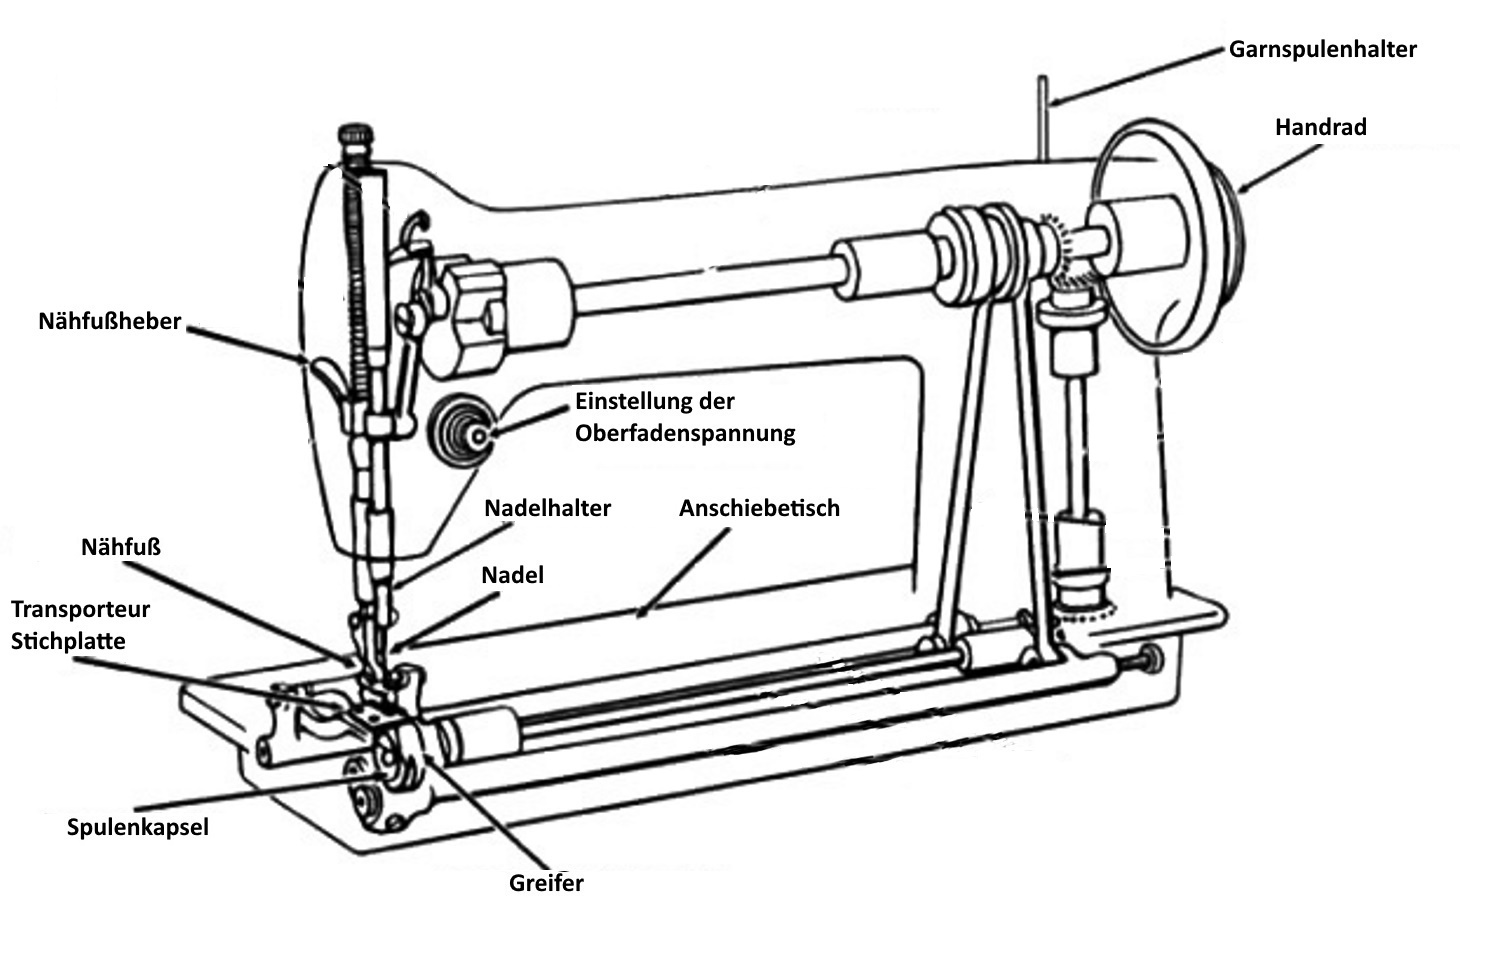
\includegraphics[width=0.8\linewidth]{naehmaschine_wichtige_teile.jpg}
\end{center}

\subsection{Nähfuß anheben und absenken}
Der Nähfuß kann mit dem Hebel an der Rückseite, links an der Maschine in zwei Positionen gebracht werden:
\begin{itemize}
	\item \textbf{abgesenkt:} Nähfußhebel ist unten, Position zum Nähen
	\item \textbf{angehoben:} Nähfußhebel ist oben, Position zum Einlegen und Entnehmen von Stoff und zum Einfädeln des Fadens
\end{itemize}

\textcolor{red}{
	\textbf{Wichtig:} Immer erst losnähen, wenn der Nähfuß abgesenkt ist. Wenn der Nähfuß noch oben ist, sind die Spannungsscheiben für den Oberfaden nicht angezogen. 
	Dadurch wird dieser viel zu weit nach unten durchgezogen. Es bildet sich ein Fadenwulst, der Stoff wird nicht mehr ordentlich transportiert und irgendwann wird auch die Nadel abbrechen. Danach wird es notwendig sein, einen großen Fadenklumpen aus dem Umlaufgreifer zu entfernen. 
	Außerdem ist die Wahrscheinlichkeit groß, dass der Stoff dabei an der Stelle, an der sich die Maschine "festgefressen" hat, ein Loch haben wird.
}

\subsection{Stichlänge einstellen}
Mit dem unteren Einstellrad auf der rechten Seite der Nähmaschine lässt sich die Stichlänge einstellen. Die Skala gibt dabei die ungefähre Stichlänge in Millimetern an.

\subsection{Rückwärts nähen}
Wenn der Hebel in der Mitte des Stichlängen-Einstellrads heruntergedrückt wird, näht die Maschine rückwärts. Das ist z.B. zum Vernähen einer Naht sehr nützlich (s.u.).
Sobald der Hebel losgelassen wird, näht die Maschine wieder vorwärts.

\subsection{Fadenspannung einstellen}
Die Einstellung der Oberfadenspannung erfolgt durch drehen am Einstellrad auf der linken Seite der Nähmaschine.
Die Fadenspannung sollte stehts so eingestellt sein, dass sich die Kreuzungspunkte des Ober- und des Unterfadens im zu nähenden Material befinden:
\begin{center}
	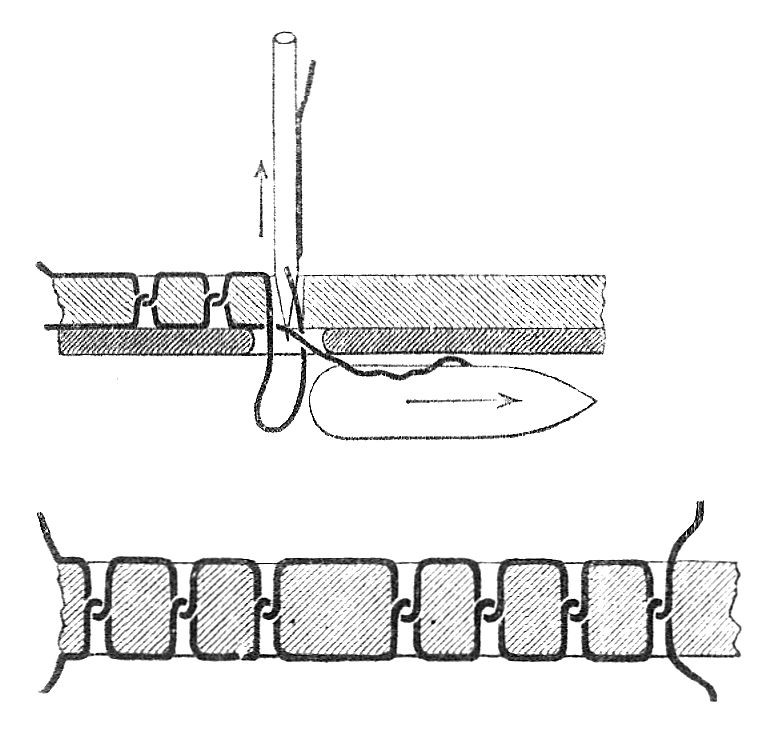
\includegraphics[width=\linewidth/2]{seam.jpg}
	\url{https://de.wikipedia.org/wiki/Datei:N%C3%A4hmaschine-Fig15und16.jpg}
\end{center}
Prinzipiell näht die Maschine mit der Oberfadenspannung in Mittelstellung (''5'') üblicherweise sehr gut.
Manche Stoffe, Garne oder Nähtechniken machen es allerdings notwendig, diese anzupassen.
Idealerweise probiert man daher vorher an einem Stück übrigem Reststoff, ob sich Unter- und Oberfaden in ''Inneren'' des Stoffes treffen oder ob einer der Fäden fälschlicherweise auf die andere Seite durchgezogen wird.
\newline
\pfeil Die Oberfadenspannung dürft ihr jederzeit euren Bedüfnissen anpassen. Bei einer gut funktionierenden Maschine sollte dies auch stets ausreichend sein. 
\newline
\textcolor{red}{\textbf{Solltet ihr dennoch das Gefühl haben, dass die Unterfadenspannung nicht korrekt eingestellt ist, korrigiert diese bitte NIEMALS selbst sondern informiert die anwesenden Betreuer:innen.}}

\subsection{Zickzack einstellen}
Neben dem normalen Geradstich, beherrscht unsere Pfaff 260 auch noch den Zickzackstich. 
Zwar haben modernere Machinen noch viele andere nützliche Stichprogramme, jedoch lassen sich mit dem nötigen Wissen schon mit diesen beiden Grundstichen quasi alle Näharbeiten erledigen. Falls du Hilfe brauchen solltest, frag einfach nach. Vielleicht kann dir jemand die entsprechenden Arbeitstechniken zeigen.  
\begin{itemize}
	\item Das obere Einstellrad an der rechten Seite der Maschine dient zur Einstellung der Breite eines permanenten Zickzackstiches. Die Skala auf dem Rad gibt die ungefähre Breite des Zickzacks in Millimetern an.
	\item Der Hebel in der Mitte des Einstellrades ermöglicht es nur momentan einen Zickzackstich zu nähen.
	Solbald der Hebel wieder losgelassen wird, wird die Maschine wieder zum Geradstich übergehen. 
	Je weiter der Hebel heruntergedrückt wird, desto breiter wird der Zickzackstich.
\end{itemize}

\subsection{Nadelposition einstellen}
Mit dem kleinen weißen Hebel unten am Zickzack-Einstellrad lässt sich die Nadelposition nach links oder rechts verstellen.
Für viele Näharbeiten ist es jedoch ausreichen, die Nadel in der Mittelposition zu belassen.
Orientiert euch am besten an der Mitte der Nähfußes, um die Nadelposition wieder in Mittelstellung zu bringen.

\subsection{Nählicht ein- und ausschalten}
Mit dem Knopf auf der rechten Seite unter dem Rückwärtshebel, lässt sich das integrierte Nählicht ein- und wieder ausschalten.

\subsection{Transporteur anheben/versenken}
Der Transporteur ist dafür zuständig, den Stoff beim Nähen automatisch weiterzuschieben. 
\newline Beim Freihandnähen, Stopfen, Sticken und Annähen von Knöpfen muss dieser versenkt werden:
\begin{itemize}
	\item Den Hebel an der Grundplatte auf der rechten Seite der Nähmaschine nach vorne, auf dich zu drehen um den Transporteur zu versenken
	\item Den Hebel wieder nach hinten, von dir weg drehen, um den Transporteur anzuheben
\end{itemize}

\subsection{Sonstiges}
\textbf{Vernähen:} 
\newline
Der Anfang und das Ende einer Naht sollten vernäht werden, damit sich diese nicht wieder von den Enden her aufdröseln kann.
Überlicherweise bewerkstelligt man das mit einer Nähmaschine, indem man unter Zuhilfenahme der Rückwärtstaste zwei- bis dreimal, 5-10mm lang auf der gleichen Stelle vor und zurück näht.
Fall die Stelle besonders gut versteckt werden soll, kann mann am Anfang und am Ende einer Naht auch ausreichend viel Faden herunterhängen lassen und die Enden anschließend mit der Hand vernähen.

\pagebreak
\section{Maschine nähbereit machen und wichtiges sonstiges Wissen}

\subsection{den richtigen Nadeltyp wählen}
\textcolor{red}{Wichtig: Unbedingt einwandfreie Nadeln verwenden: gute Qualität, gerade, nicht verbogen oder abgebrochen, schlägt nicht an, usw.!}
Zudem muss es sich stets um Flackolbennadeln (Art 130/705H) handeln.
\newline


Viele Näharbeiten können mit einer sogenannten Universalnadel durchgeführt werden. Für manche Stoffe und Nahtarten benötigt man jedoch spzielle Nadeltypen.
So gibt es z.B. Stretch- u. Jerseynadeln (rundere Spitze, um den feineren Stoff nicht zu zerstechen), Jeansnadeln, Microtexnadeln, Zwillingsnadeln, usw. 
\newline


Unten seht ihr eine unvollständige Liste verschiedener Nadeltypen:
\begin{center}
	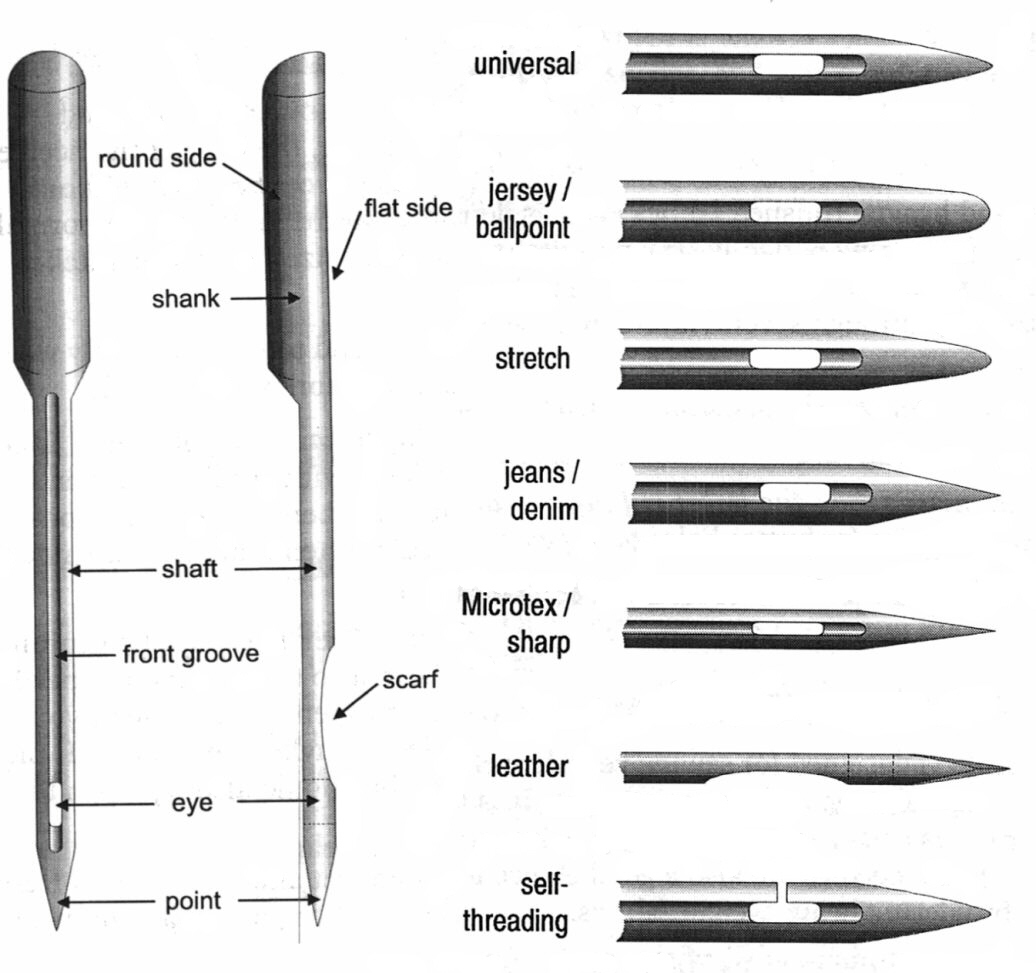
\includegraphics[width=\linewidth/2]{Sewing-machine-needles-types.jpg}
	\url{https://de.wikipedia.org/wiki/Datei:Sewing-machine-needles-types.jpg}
\end{center}

\subsection{Nadeln wechseln}
\begin{enumerate}
	\item Die Nadel mit dem Handrad in höchste Stellung bringen
	\item Nähfuß absenken
	\item Schraube rechts an Nadel ca. eine halbe Umdrehung öffnen
	\item Nadel entfernen (nicht einfach herausfallenlassen, sondern herausnehmen)
	\item Nadel mit abgeflachter Seite nach hinten einlegen
	\item Neue Nadel in Halterung einführen und bis zum Anschlag nach oben schieben
	\item Schraube festdrehen - fest, aber ohne Gewalt
\end{enumerate}

\subsection{Nähfuß wechseln}
Es gibt verschiedene Nähfüße, je nach Einsatzweck können diese ausgewechselt werden. Es gibt z.B. Stopffüße, Stickfüße, Bandeinfasser, Freihandfüße, Teflonfüße usw. 

\begin{enumerate}
	\item Die Nadel mit dem Handrad in höchste Stellung bringen
	\item Nähfuß anheben
	\item Näfußschraube an der linken Seite der Nadelstange lösen
	\item Nähfuß abnehmen
	\item Neuen Nähfuß anbringen
	\item Näfußschraube wieder festziehen - fest, aber ohne Gewalt
\end{enumerate}

\subsection{Oberfaden einfädeln}
\textcolor{red}{Nur bei angehobenem Fuß, da sonst die Spannungsscheiben zusammengedrückt sind und der Faden nicht korrekt dazwischen gefädelt werden kann!}
\newline

\begin{enumerate}
	\item Fadenhebel mit Handrad in höchste Position bringen
	\item Garnrolle auf Garnrollenhalter stecken
	\item Faden durch Führung über dem Oberfandenspannungs-Einstellrad durch eines der Löcher führen
	\item Einmal um das Spannungsrad in einer der beiden Führungen herumführen und nach rechts ziehen, damit der Faden unter und hinter den Führungsdorn an der Oberseite des Spannungsrades rutscht 
	\item Garn durch eines der Löcher im Fadenhebel führen
	\item Durch die beiden Führungsösen Richtung Nadel führen (Garn kann von der linken Seite in die Führungsösen gezogen werden)
	\item Faden in die Öse der Nadel einfädeln (manuell oder mit der Nadeleinfädler)
\end{enumerate}

\vspace{2em}

\textbf{Test auf richtiges Einfädeln:}
\begin{enumerate}
 \item Einfädeln
 \item Nähfuß angehoben lassen
 \item den Faden leicht nach hinten weg ziehen \pfeil wenig/kein Widerstand!
 \item Nähfuß absenken
 \item den Faden leicht nach hinten weg ziehen \pfeil Widerstand, Nadel biegt sich leicht (nicht gegen Widerstand ziehen!)
\end{enumerate}
Falls sich der Faden sowohl mit abgesenkten wie auch mit angehobenem Nähfuß jeweils beide Male leicht oder schwer wegziehen lässt ist der Faden nicht richtig eingefädelt.
\newline
\textcolor{red}{\pfeil In diesem Fall bitte den Faden noch einmal komplett herausziehen und neu einfädeln.} 

\subsection{Unterfaden aufspulen}
Obwohl man den Unterfaden idealerweise nicht an der Oberseite eines Nähstücks sehen wird, verwendet man dafür üblicherweise das gleiche Garn wie für den Unterfaden.
Verwendet man verschiedene Garne, so sollte der Unterfaden stets höchstens so stark wie oder etwas schwächer als der Oberfaden sein.
Es ist daher notwendig ein Stück Garn von der Garnrolle auf eine kleinere Unterfadenrolle zu spulen.

\begin{enumerate}
	\item Passende Spulen verwenden (sind vorhanden)
	\item Spule auf den Rollenhalter rechts oben auf der Maschine stecken, so dass diese in den kleinen Metallstift einrastet
	\item Spulhebel neben der Spule richtung Spule drücken
	\item Faden von Garnrolle in Uhrzeigersinn um den Spannungsknopf führen (Faden kreuzt sich)
	\item Faden ein paar Mal um Spule wickeln
	\item Fadenende locker festhalten, Fußanlasser drücken, Faden wird aufgespult (Faden dabei loslassen)
	\item Wenn die Spule voll ist, schaltet sich der Spuler automatisch ab
	\item Faden abschneiden, Spule abnehmen
\end{enumerate}

\subsection{Unterfaden heraufholen}
\begin{enumerate}
	\item Oberfaden mit der linken Hand am Ende festhalten und leichten Zug auf diesen ausüben
	\item Der Greifer wird den Oberfaden ab einem bestimmten Punkt nach unten ziehen (weiter festhalten!)
	\item Unter konstantem leichten Zug am Oberfaden Handrad auf dich zu drehen
	\item Irgendwann kommt der Unterfaden zum Vorschein
	\item Handrad soweit weiterdrehen, bis der Oberfaden wieder vollständig oberhalb der Stichplatte ist
	\item Falls das Ende des Unterfadens noch nicht zu sehen ist, dieses mit einer Nadel oder einer kleinen Schere nach oben ziehen
\end{enumerate}

\subsection{Unterfaden heraufholen}
\begin{enumerate}
	\item Je nach Nähfuß, Oberfaden durch den Schlitz in der Mitte des Näfußes führen
	\item Beide Fäden nach hinten führen un hinten an der Maschine herunterhängen lassen
	\item Beide Fäden nicht zu kurz abschneiden (mindestens 5-10cm lan lassen)
\end{enumerate}

\subsection{Unterfaden einfädeln}

Am besten ist es, der bebilderten Anleitung im Handbuch zu folgen.

\vspace{1em}
\begin{enumerate}
 \item Nadel in die höchste Position bringen
 \item Maschine vorsichtig nach hinten kippen (\textcolor{red}{Maschine ist schwer und fällt leicht nach hinten um! Die Maschine ist nicht fest am unteren Holzkasten befestigt und kann \enquote{herausfallen}.})
 \item Spulenkapsel herausnehmen
 \item Evtl. noch vorhandene Spule entfernen
 \item Neue Spule einsetzen (Faden muss sich in Richtung des schrägen Schlitzes in der Spulenkasel abrollen, gegen den Uhrzeigersinn)
 \item Faden in den Schlitz und unter das Spannungsblech ziehen (Faden sollte ca. 10-15cm aus der Kapsel heraushängen)
 \item Spulenkasel in linke Hand nehmen und Hebel daran zur Seite ziehen, damit die Spule nicht herausfällt
 \item Mit der rechten Hand die Maschine wieder ankippen
 \item Spule so einsetzen dass die Spitze des kleinen Hebels waagerecht nach rechts zeigt
 \item Spulenkapsel vollständig wieder in Greifer einschieben
 \item Hebel loslassen
\end{enumerate}

% schoenere Darstellung
\newpage
\ccLicense{naehmaschine-einweisung}{Einweisung Nähmaschine}

\end{document}
